\documentclass[12pt]{article}
\usepackage{geometry}                
\geometry{letterpaper}                   % ... or a4paper or a5paper or ... 
\usepackage[parfill]{parskip}    
\usepackage{graphicx}
\usepackage{amssymb}
\usepackage{amsmath}
\usepackage{hyperref}

\usepackage[usenames,dvipsnames,svgnames,table]{xcolor}

\hyphenpenalty=10000

\title{Sequencing Uncertainty Propagation}
\author{David Champredon}
\date{\today}                                           % Activate to display a given date or no date

\newcommand{\comment}[1]{\textsl{\textcolor{cyan}{#1}}}
\newcommand{\sq}[1]{\texttt{\textcolor{brown}{#1}}}
\newcommand{\pr}[1]{\mathrm{Pr}(#1)}


\begin{document}
\maketitle

\section{Background}

Identifying the sequence of nucleotides from a biological sample is a complex process which is fraught with noise. 

Assuming the biological sample of interest has been properly isolated (that is it is complete, has no damages or contamination), sequencing a biological sample, whether with the Sanger method or ``Next-Generation Sequencing'' (NGS) usually involves:
\begin{itemize}
\item if the sample of interest is RNA: Reverse transcription 
\item DNA fragmentation in smaller pieces than the original sample (less than 400bp for NGS, 800bp for Sanger)
\item amplification of the fragmented DNA using PCR
\item sequencing the fragments (identifying the nucleotides from a fluorescent tag attached)
\item alignment or mapping: putting back the small fragment together by aligning them (de novo) or mapping them on benchmark libraries
\end{itemize}


Errors can be introduced at each of these steps for various reasons \cite{Beerenwinkel:2011}. It is probably not feasible to determine what is the source of the noise, nor to try to eliminate it completely.
The goal here is to acknowledge there is uncertainty in the output sequence given from any sequencing method and to propose a method to propagate this uncertainty in any downstream analysis.
Currently, this uncertainty is recognized and even quantified with sequencing quality scores (FASTQ files), but it does not seem those scores are used to inform a probabilistic model to represent the sequence. 
Simply put, we shouldn't treat the result of sequencing as a \emph{certainty}.




\section{Probabilistic representation}

\subsection{Definition}
 
We can represent probabilistically a nucleotide sequence in a matrix form. For a sequence of length $\ell$ we can write:

$$S = \bordermatrix{   & 1 & 2 & \ldots & \ell \cr
                \sq{A} & p_{A, 1} & p_{A, 2} & \ldots & p_{A, \ell} \cr
                \sq{C} & p_{C, 1} & p_{C, 2} & \ldots & p_{C, \ell} \cr
                \sq{G} & p_{G, 1} & p_{G, 2} & \ldots & p_{G, \ell} \cr
                \sq{T} & p_{T, 1} & p_{T, 2} & \ldots & p_{T, \ell} \cr 
                \sq{x} & p_{x, 1} & p_{x, 2} & \ldots & p_{x, \ell} \cr 
}$$

Each column represents the nucleotide position, each row one of the four nucleotide \sq{A,C,G,T} as well as an empty position \sq{x}.
Hence, $S$ is a $5\times\ell$ matrix. Its elements represent the probability that a nucleotide is at given position:

\begin{equation}
S_{n,j} = \pr{\text{nucleotide \sq{n} is at position }j}
\end{equation}
with the special case for a deletion:

\begin{equation}
S_{\sq{x},j} = \pr{\text{empty position }j}
\end{equation}

The matrix $S$ will be called the \emph{probabilistic sequence} of a biological sample.
Note, that we have, for all $1\leq j \leq \ell$:
\begin{equation}
\sum_{n\in \{ \sq{A,C,G,T,x} \} } S_{n, j} = 1
\end{equation}

The sequence of nucleotides from a biological sample is not treated as certainty anymore, but as a collection of possible sequences, with length not necessarily equal when the probability of an empty position is positive. 



\subsection{Examples}

If we have the following probabilistic sequence
$$
S = 
\begin{pmatrix}
0.9 & 0.05   & 0.99 & 0 & 0\\
0   & 0.8 & 0 & 0 & 0.1\\
0.1 & 0.15 & 0 & 0.3 & 0.9\\
0 & 0 & 0.01 & 0.7 & 0\\
0 & 0 & 0 & 0 & 0\\
\end{pmatrix}
$$
then there are $2\times 3 \times 2^3 = 48$ possible sequences. The most likely is the one having the highest nucleotides probabilities: \sq{ACATG} with probability 0.449  ($0.9\times 0.8\times 0.99 \times 0.7 \times 0.9$).

If there is a positive probability for at least one empty position, then the sequence has a variable length. 
Let's take the same example as above, but adding one possible empty position:

$$
S = 
\begin{pmatrix}
0.9 & 0.05   & 0.99 & 0 & 0\\
0   & 0.8 & 0 & 0 & 0.1\\
0.1 & 0.15 & 0 & 0.2 & 0.9\\
0 & 0 & 0.01 & 0.7 & 0\\
0 & 0 & 0 & 0.1 & 0\\
\end{pmatrix}
$$

Like above, there is still a 0.449 probability that the sequence is \sq{ACATG}, but with probability 0.064, the sequence could be shorter when position 4 is empty and be \sq{ACAG}.



\section{Quantifying probabilities}

The difficulty of estimating the probabilities that populate the probabilistic sequence lies in quantifying errors at each steps (fragmentation, amplification, sequencing, alignment). And how to integrate these error types in a coherent fashion?


\subsection{Sequencing errors}

Maybe the easiest error type to quantify is the fragment sequencing error because a quality (or ``Phred'') score is attributed to each base call. The quality score $Q$ is directly related to the error probability: $p = 10^{-Q/10}$ (\autoref{fig:phred}). 

\begin{figure}[ht]
\begin{center}
 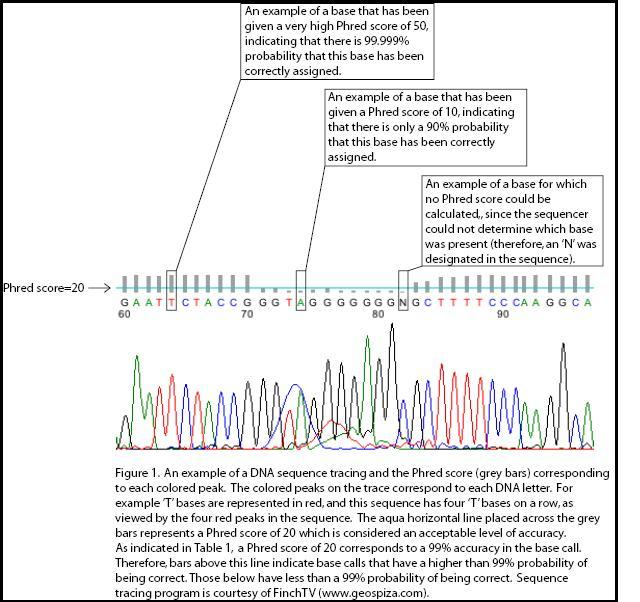
\includegraphics[width = 0.9\textwidth]{figs/Phred.jpg}
\caption{Example of quality scores associated with a chromatograph.}
\label{fig:phred}
\end{center}
\end{figure}

As I don't have FASTQ files from actual biological samples, I use the software  \textsf{inSilicoSeq} that simulates the sequencing of short reads from Illumina instruments. 
As shown in \autoref{fig:probaErrISS}, the sequencing error probability ranges between $10^{-3.5}$ and  $10^{-1.5}$.  

\begin{figure}[ht]
\begin{center}
 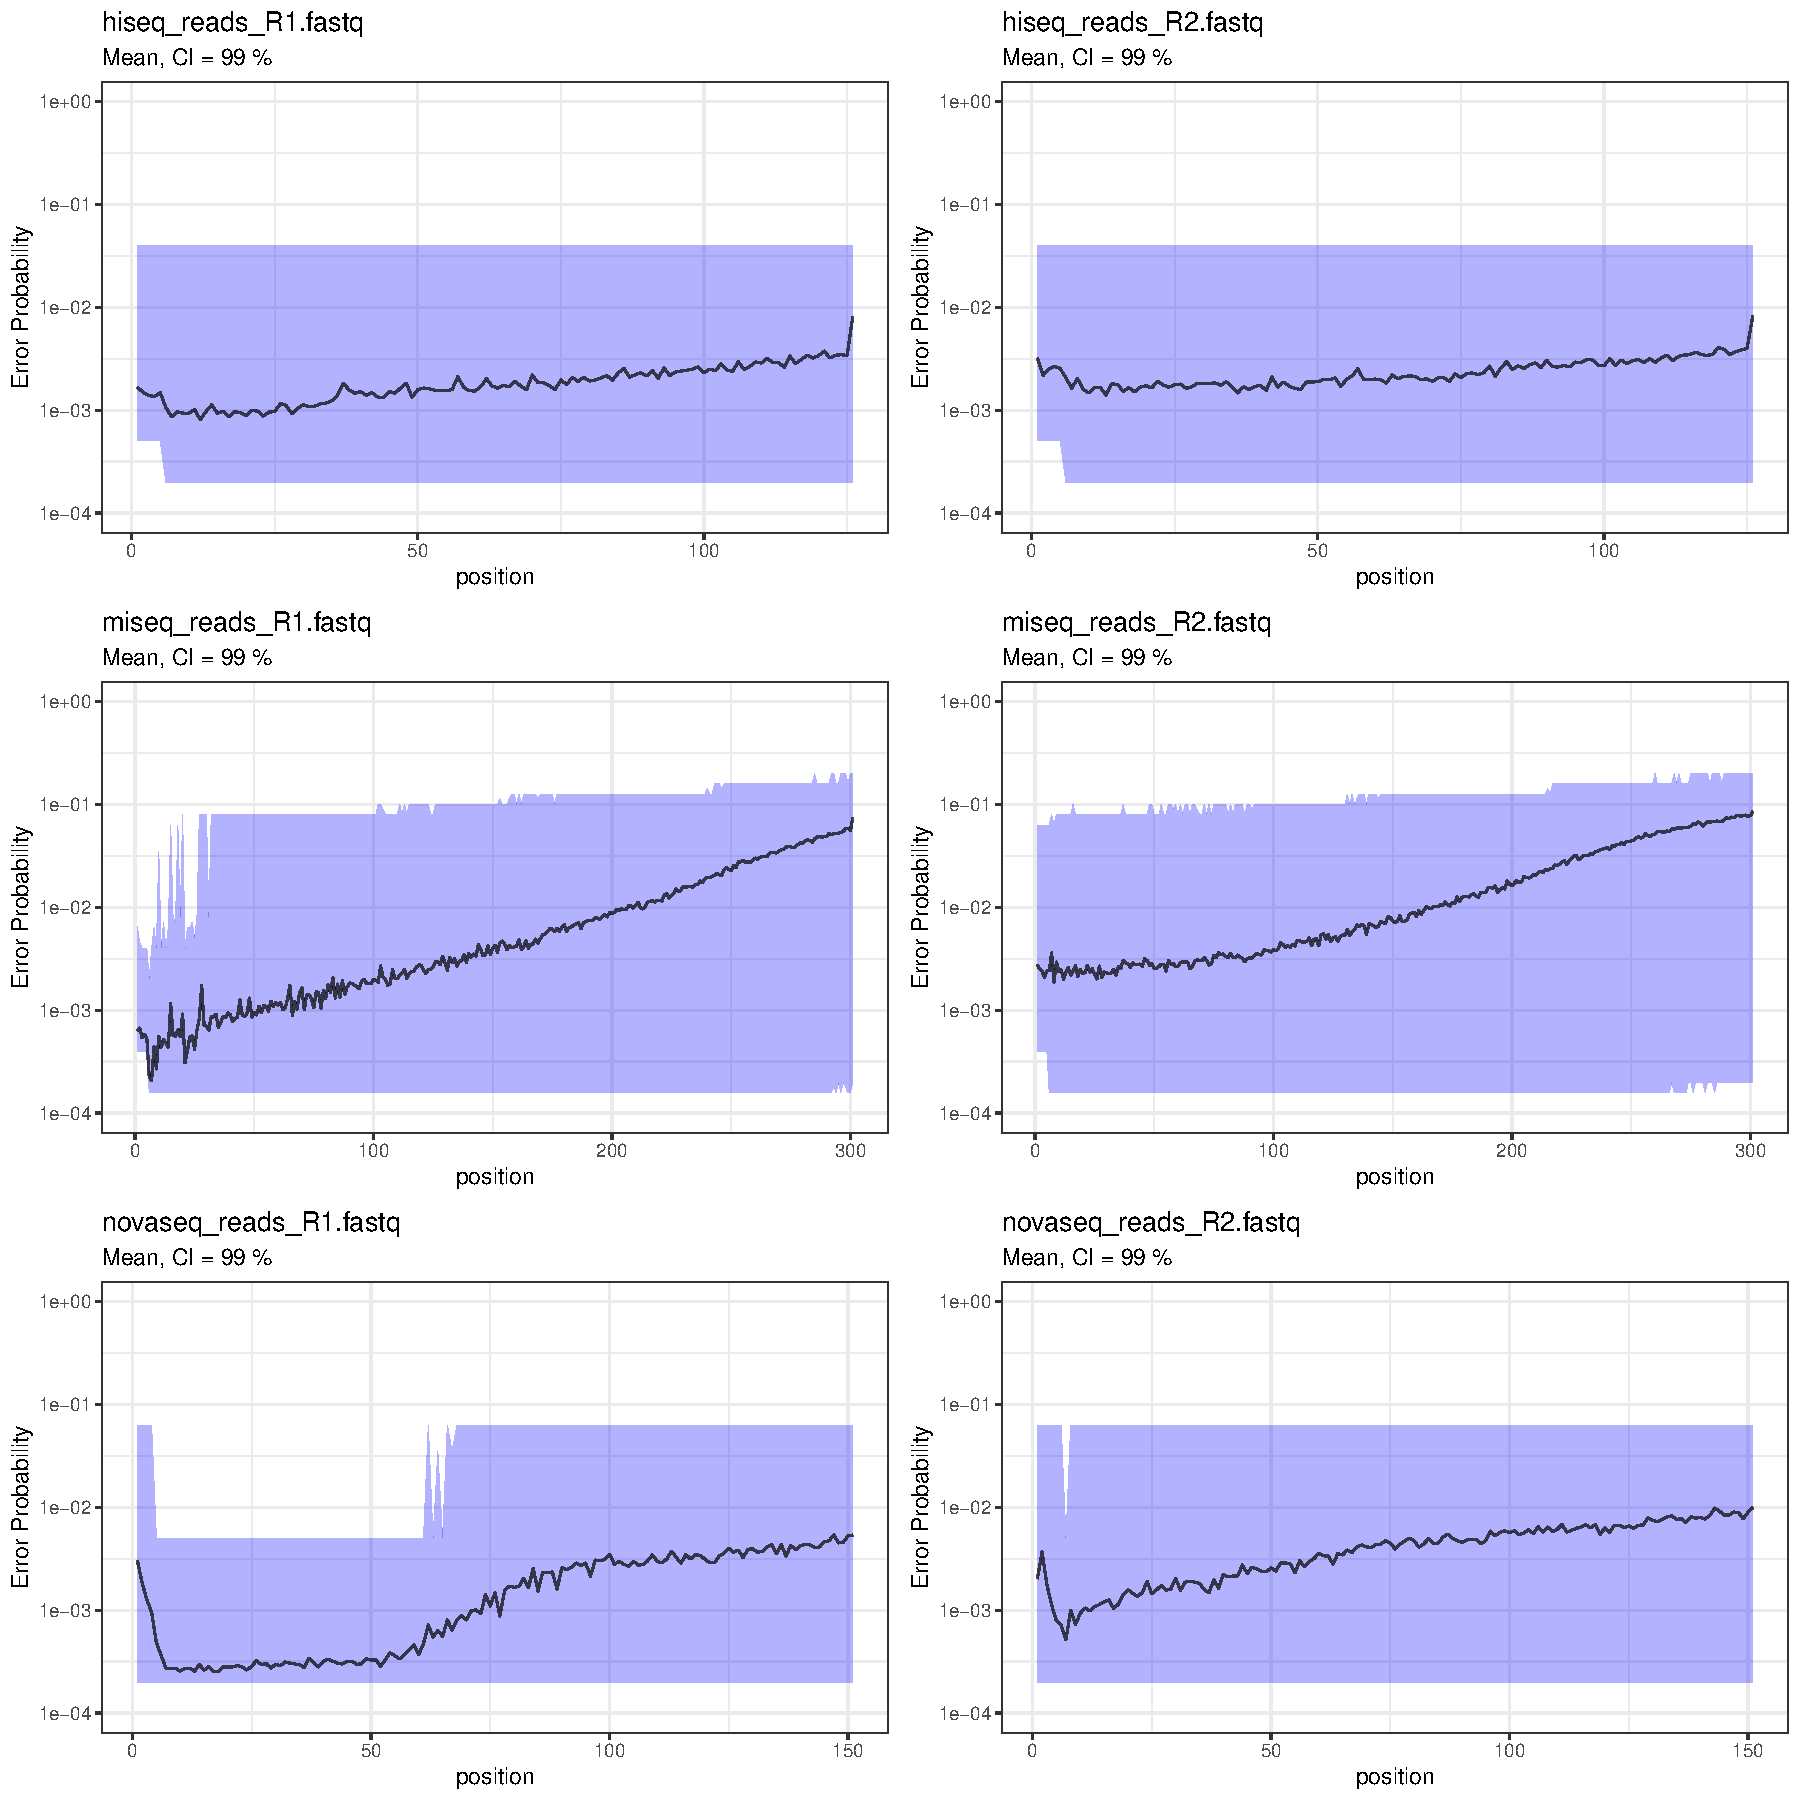
\includegraphics[width = 0.99\textwidth]{figs/plot-errorProba.pdf}
\caption{Error probability of calling bases for 3 different Illumina instruments (HiSeq, MiSeq, NovaSeq) simulated with \textsf{InSilicoSeeq}. Figure generated by running \texttt{reads-seq-err/go.sh}.}
\label{fig:probaErrISS}
\end{center}
\end{figure}

After alignment, taking an optimistic view, we can assume a unique global sequencing error of $\epsilon=10^{-3.5}=0.0003$.
So each base call is right with probability $1-\epsilon$. Assume the other bases and missing position \sq{x} are all equally likely with probability $(1-\epsilon)/4$. 

For example, if the output sequence after fragment sequencing and alignment is \sq{ACGT} the probabilistic sequence is:

$$
S = 
\begin{pmatrix}
1-\epsilon & \epsilon/4    & \epsilon/4  & \epsilon/4  \\
\epsilon/4 & 1-\epsilon & \epsilon/4  & \epsilon/4  \\
\epsilon/4 & \epsilon/4  & 1-\epsilon  & \epsilon/4 \\
\epsilon/4 & \epsilon/4  & \epsilon/4  & 1-\epsilon \\
\epsilon/4 & \epsilon/4  & \epsilon/4  & \epsilon/4 \\
\end{pmatrix}
$$

\subsection{Polymorphism, in-host diversity}

The probabilistic sequence can also be interpreted as a representation of polymorphism abundance in a biological sample from one single host (in-host diversity).

There may be one problem: the data will give abundances of several sequences -- say 10 -- found in one host. 
When sampling from the probabilistic sequence, it is not constraint to a given number of specific sequences. For a sequence of length $n$ the number of  unique sequences is $5^n$. Even if we do not observe perfectly, it is almost sure that the real diversity is a minute fraction of the $5^n$ possible sequences.
 
Maybe this can be overcome by thinking in terms of diversity \emph{and} sequencing error.
In that case the probabilities would be defined primarily for the diversity and another smaller layer for sequencing error. 

Not too sure about all that... 


\section{Sequence logo and entropy}

Are sequence logos along with their entropy calculation a better start than the probabilistic sequence? 

Schneider \cite{Schneider:1986,schneider1990sequence,Schneider:2002} used information theory, Shannon entropy, to quantify the uncertainty in ``bits''. Is that better? 

The bits are the number of binary digits, i.e., 0 or 1, needed to translate the possibilities of a ``message''. Here the message is a base call, or rather bases associated with their probabilities. 
The larger the number of bits required to translate the message, the more uncertain. 
In my mind, uncertainty and entropy are similar, the only important difference is that entropy is quantified in bits. 

The entropy (i.e., uncertainty) at a given position $j$ is given by Shannon's standard expression:

\begin{equation}
H = -\sum_{n\in\{\sq{A,C,G,T}\}} S_{n,j}\log_2(S_{n,j})
\end{equation}
with, as before, $S_{n,j}$ being the probability that nucleotide $n$ is at position $j$.

For example, if we know for sure that the nucleotide at a given position is \sq{C}, that is $S_{\sq{C},j}=1$, then entropy (uncertainty) is $H=0$: we don't need any bit to translate that \sq{C} is at this position, it's sure, we know that. 

Another example, is when any of the four bases are equally likely. All probabilities are 1/4, and the entropy is maximum with a value $H = 2$ bits ($=-4\times \frac{1}{4}\times \log_2(\frac{1}{4})$). 
  
I'm not sure how useful Schneider's $R_{sequence}$ metric is in my case (propagating uncertainty in tree reconstruction).
The entropy $H$ may be more useful as a principled measure of uncertainty at a given position. 
 
\newpage

\bibliographystyle{plain}
\bibliography{papers}

\end{document}  